This section will give an overview of ear-decomposition and Mondshein-sequences.
\subsection{Ear Decomposition}
\begin{defn}\label{def:eardecomp}
An \textit{ear decomposition} of a 2-connected graph $G=(V,E)$ is a decomposition $G = (P_0, P_1,... P_K)$ that partitions E,
where $P_0$  is a cycle and $P_i, 1 \leq i \leq K$ is a path with only its two distinct end vertices in common with $(P_0 \cup P_1 \cup ... \cup P_{i-1})$. 
Each $P_i$ is called an \textit{ear}.
\end{defn}

\begin{figure}
    \centering
    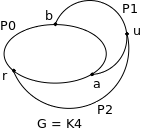
\includegraphics[scale=0.6]{earDecomp.png} \\
    \caption{An example of ear decomposition of a $K_4$ containing 3 ears.}
    \label{fig:earDecomp}
\end{figure}

Now we will define some terms associated with an ear decomposition.
An \textit{ear} is called \textit{short} if it is an edge and \textit{long} otherwise.
For any $i$, let $G_i = (P_0 \cup P_1 \cup ... \cup P_{i})$ and $\overline{V_i} := V - V(G_i)$, and $\overline{G_i}$ is a graph induced by $\overline{V_i}$.
Note that, $\overline{G_i}$ does not necessarily contain all edges in $E - E(G_i)$, there can be short ears which have both the end points in $G_i$.
For a path $P$ and two of its vertices $x$ and $y$, $P[x,y]$ be the sub-path in P from $x$ to $y$.
A path with endpoints $v$ and $w$ is called a \textit{vw-path}.
A vertex $x$ in a \textit{vw-path} is called an \textit{inner vertex} if $x \notin \{v,w\}$.
For simplicity we assume that every vertex in $P_0$ is an inner vertex.
\textit{inner(P)} denotes a set of inner vertices of an ear P.
For an edge $e \in G$, $birth(e)$ is the index $i$ where $e$ is born, i.e. $i$ such that $P_i$ contains $e$.
Similarly, for a vertex $v \in G$, $birth(v)$ is the index $i$ of the first path $P_i$ that contains $v$, 
in other words, $P_{birth(v)}$ is the ear containing $v$ as an inner vertex.

\begin{defn}\label{def:nonseperating}
Let $D = (P_0, P_1,... P_K)$ be an ear decomposition of G.
D is defined as a \textit{non-separating} ear decomposition if, for all $i, 0 \leq i \leq k$, $\overline{G_i}$ is connected  
and each internal vertex of ear $P_i$ has a neighbor in $\overline{G_i}$.
\end{defn}

We will now see how canonical ordering for a plane graph can be expressed using a non-separating ear decomposition.

\begin{defn}\label{def:canonical}
Canonical ordering (another definition).
Let G be a 3-connected plane graph having edges $v_1v_2$ and $v_2v_n$ on its outer face.
A \textit{canonical ordering} with respect to $v_1v_2$ and $v_2v_n$ is an ear decomposition D of G such that:
\begin{enumerate}
\item $v_1v_2 \in P_0$,
\item $P_{birth(v_n)}$ is the last long ear, that contains $v_n$ as its only inner vertex and does not contain $v_2v_n$, and
\item D is non-separating.
\end{enumerate}
\end{defn}

\textit{How is the above definition similar to old definition (Def. 8.1 in lecture notes) of canonical ordering?}
Recall, old definition (Def 8.1 in lecture notes) also had $v_1,v_2,v_n$ fixed on the outer triangular face.
Edge $v_1v_2$ was first fixed on the outer face and we incrementally formed G by adding $v_{k+1}$ to $G_k$ at each step.
Vertex $v_{k+1}$ was adjacent to two or more outer-face vertices of $G_k$, in other words $G_k$ was connected to $\overline{G_k}$, hence property 3 makes sense.
Vertex $v_n$ was added at last, one can imagine arc $v_1v_nv_i$, $i \notin \{1,2,n\}$ as a last long ear where $v_n$ is an inner vertex.
The difference (between Def \ref {def:canonical} and Def 8.1 in lecture notes) lies in property 2, remember that in lecture we saw canonical ordering for a triangulated graphs, 
but Def. \ref{def:canonical} is for any 3-connected graph, therefore vertex $v_n$ should have degree at least three.
Hence, long ear $P_{birth(v_n)}$ cannot contain $v_2v_n$; $v_2v_n$ should be a short ear.
It is also evident that adding vertex $v_3$ forms a cycle $v_1v_2v_3$, think of it as $P_0$ in the above definition.


\subsection{Mondshein sequence}
Now we will see how can Definition \ref{def:canonical} be extended for non-planar graphs.
Notice that Definition \ref{def:canonical} uses planarity only at one place: we assumed edges $v_1v_2$ and $v_2v_n$ are on the outer face.
By dropping this assumption we can generalize Definition \ref{def:canonical} for non-planar graphs, all we need is that $v_1v_2$ and $v_2v_n$ should be edges in graph G.

In 1971, Mondshein used a similar definition to define a $(2,1)-sequence$ [\cite{mond} Def. 2.2.1], but it was in the notation of a special vertex ordering.
For conciseness, we will stick to the ear-decomposition based definition in these notes, which is similar to the one given by Cheriyan \cite{cheriyan}.

\begin{defn}\label{def:mond}
(\cite{mond}, \cite{cheriyan}). Let G be a graph with an edge $v_2v_n$. A \textit{Mondshein sequence avoiding $v_2v_n$} is an ear decomposition D of G such that:
\begin{enumerate}
\item $v_2 \in P_0$
\item $P_{birth(v_n)}$ is the last long ear, that contains $v_n$ as its only inner vertex and does not contain $v_2v_n$, and
\item D is non-separating.
\end{enumerate}
\end{defn}

In other words the edge $v_2v_n$ is added last in D as a short ear, right after the last long ear $P_{birth(v_n)}$ has been added, and as a direct consequence of property (2) and (3), 
G must have a minimum degree 3 to have a Mondshein sequence.
This has also been explained after Def. \ref{def:canonical}.
Moreover, Mondshein in his thesis \cite{mond} proved that every 3-connected graph has a Mondshein sequence.
\textit{If D satisfies property (1) and (2) it is said to avoid $v_2v_n$.}
